\chapter{Branch-and-Bound Algorithms}
\label{chapter:branch-and-bound}

\abstract{
One of the earliest approaches to the top-$k$ retrieval problem
is to partition the vector space recursively into smaller regions
and, each time we do so, make note of their geometry.
During search, we eliminate the regions
whose shape indicates they cannot contain or overlap with the solution set.
This chapter covers algorithms that embody this approach
and discusses their exact and approximate variants.
}

\section{Intuition}
\label{section:branch-and-bound:intuition}

Suppose there was some way to split a collection $\mathcal{X}$ into
two sub-collections, $\mathcal{X}_l$ and $\mathcal{X}_r$, such that
$\mathcal{X} = \mathcal{X}_l \cup \mathcal{X}_r$ and that the two
sub-collections have roughly the same size. In general, we can relax the splitting
criterion so the two sub-collections are not necessarily partitions; that is,
we may have $\mathcal{X}_l \cap \mathcal{X}_r \neq \emptyset$. We may also
split the collection into more than two sub-collections. For the moment,
though, assume we have two sub-collections that do not overlap.

Suppose further that, we could geometrically characterize \emph{exactly} the regions that contain
$\mathcal{X}_l$ and $\mathcal{X}_r$. For example, when $\mathcal{X}_l \cap \mathcal{X}_r = \emptyset$,
these regions partition the space and may therefore be characterized by a separating hyperplane.
Call these regions $\mathcal{R}_l$ and $\mathcal{R}_r$, respectively.
The separating hyperplane forms a \emph{decision boundary} that helps us determine
if a vector falls into $\mathcal{R}_l$ or $\mathcal{R}_r$.

In effect, we have created a binary tree of depth $1$ where the root node has a decision boundary
and each of the two leaves contains data points that fall into its region.
This is illustrated in Figure~\subref*{figure:branch-and-bound:motivation:single-split}.

Now suppose we have a query point $q$ somewhere in the space and that we are interested
in finding the top-$1$ data point with respect to a proper distance function $\delta(\cdot, \cdot)$.
$q$ falls either in $\mathcal{R}_l$ or $\mathcal{R}_r$;
suppose it is in $\mathcal{R}_l$. We determine that by evaluating the decision boundary in the 
root of the tree and navigating to the appropriate leaf.
Now, we solve the exact top-$1$ retrieval problem over $\mathcal{X}_l$
to obtain the optimal point in that region $u_l^\ast$, then make a note of this minimum distance obtained,
$\delta(q, u_l^\ast)$.

\begin{figure}[t]
    \centering
    \subfloat[]{
        \label{figure:branch-and-bound:motivation:single-split}
        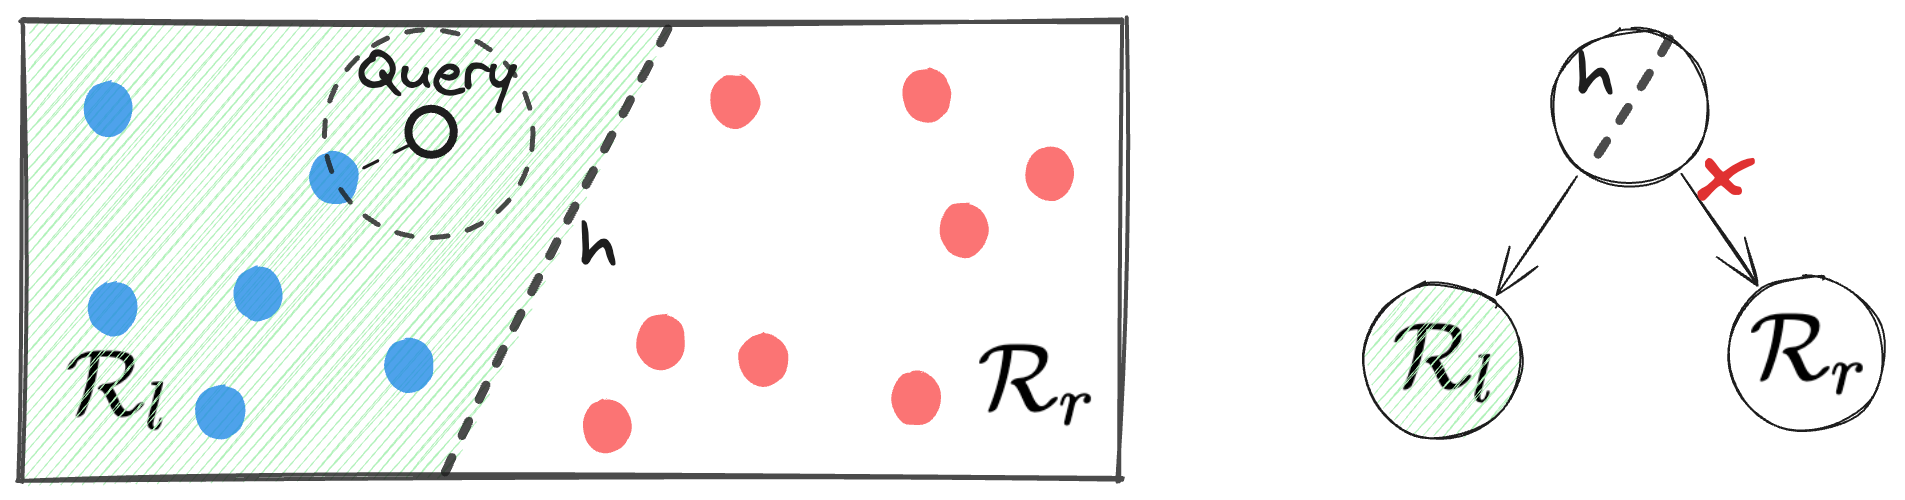
\includegraphics[width=0.7\linewidth]{figures/branch-and-bound-motivation.png}
    }

    \subfloat[]{
        \label{figure:branch-and-bound:motivation:multiple-split}
        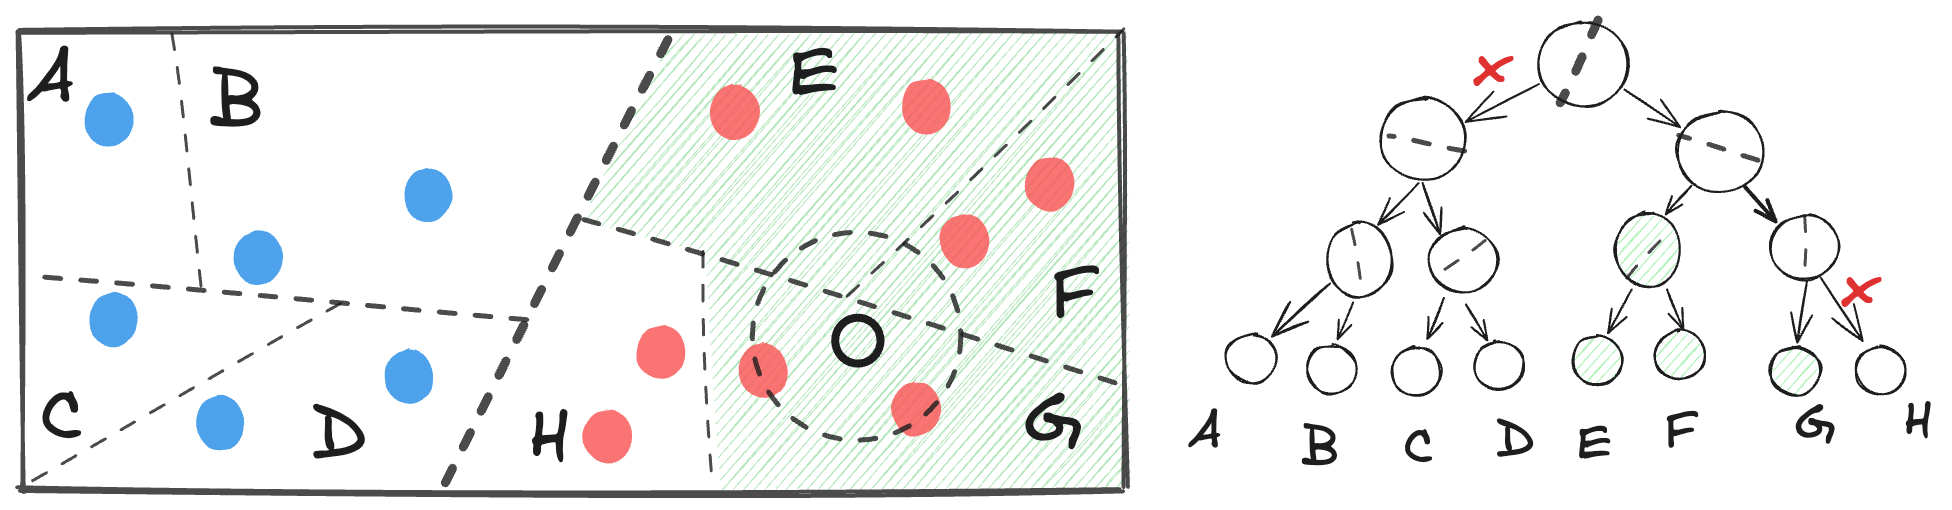
\includegraphics[width=0.7\linewidth]{figures/branch-and-bound-motivation-multiple-splits.png}
    }
    \caption{Illustration of a general branch-and-bound method on a toy collection in $\mathbb{R}^2$.
    In (a), $\mathcal{R}_l$ and $\mathcal{R}_r$ are separated by the dashed line $h$.
    The distance between query $q$ and the closest vector in $\mathcal{R}_l$ is less than the distance between $q$ and
    $h$. As such, we do not need to search for the top-$1$ vector
    over the points in $\mathcal{R}_r$, so that the right branch of the tree is pruned.
    In (b), the regions are recursively split until each
    terminal region contains at most two data points.
    We then find the distance between $q$ and the data points in the region that contains $q$, $G$.
    If the ball around $q$ with this distance as its radius does not intersect a region, we can safely prune
    that region---regions that are not shaded in the figure.
    Otherwise, we may have to search it during the certification process.}
    \label{figure:branch-and-bound:motivation}
\end{figure}

At this point, if it turns out that $\delta(q, u_l^\ast) < \delta(q, \mathcal{R}_r)$\footnote{
The distance between a point $u$ and a set $\mathcal{S}$ is defined as
$\delta(u, \mathcal{S}) = \inf_{v \in \mathcal{S}} \delta(u, v)$.}
then we have found the optimal point and do not need to search the data points in $\mathcal{X}_r$ at all!
That is because, the $\delta$-ball\footnote{The ball centered at $u$ with radius $r$ with respect to metric $\delta$
is $\{ x \;|\; \delta(u, x) \leq r \}$.}
centered at $q$ with radius $\delta(q, u_l^\ast)$ is contained entirely in $\mathcal{R}_l$,
so that no point from $\mathcal{R}_r$ can have a shorter distance to $q$ than $u_l^\ast$.
Refer again to Figure~\subref*{figure:branch-and-bound:motivation:single-split} for an
illustration of this scenario.

If, on the other hand, $\delta(q, u_l^\ast) \geq \delta(q, \mathcal{R}_r)$, then
we proceed to solve the top-$1$ problem over $\mathcal{X}_r$ as well and
compare the solution with $u_l^\ast$ to find the optimal vector.
We can think of the comparison between $\delta(q, u_l^\ast)$ with $\delta(q, \mathcal{R}_r)$
as backtracking to the parent node of $\mathcal{R}_l$ in the equivalent tree---which is the root---and comparing
$\delta(q, u_l^\ast)$ with the distance of $q$ with the decision boundary.
This process of backtracking and deciding to prune a branch or search it
\emph{certifies} that $u_l^\ast$ is indeed optimal, thereby solving the top-$1$ problem exactly.

We can extend the framework above easily by recursively splitting the two sub-collections
and characterizing the regions containing the resulting partitions. This leads to a (balanced)
binary tree where each internal node has a decision boundary---the separating hyperplane of its child regions.
We may stop splitting a node if it has fewer than $m_\circ$ points.
This extension is rendered in Figure~\subref*{figure:branch-and-bound:motivation:multiple-split}.

The retrieval process is the same but needs a little more care:
Let the query $q$ traverse the tree from root to leaf,
where each internal node determines if $q$ belongs to
the ``left'' or ``right'' sub-regions and \emph{routes} $q$ accordingly.
Once we have found the leaf (terminal) region that contains $q$, we find the
candidate vector $u^\ast$, then backtrack and certify that $u^\ast$ is indeed optimal.

During the backtracking, at each internal node, we compare the distance between $q$ and
the current candidate with the distance between $q$ and the region on the other side of
the decision boundary. As before, that comparison results in either pruning a branch or searching it
to find a possibly better candidate. The certification process stops when we find ourselves
back in the root node with no more branches to verify, at which point we have found the optimal solution.

The above is the logic that is at the core of branch-and-bound algorithms for top-$k$
retrieval~\citep{dasgupta2015rptrees,kdtree,ram2019revisiting_kdtree,mtrees,vptrees,liu2004SpillTree,panigrahy2008improved-kdtree,conetrees,xbox-tree}.
The specific instances of this framework differ in terms of how they
\emph{split} a collection and the details of the \emph{certification} process.
We will review key algorithms that belong to this family in the remainder of this chapter.
We emphasize that, most branch-and-bound algorithms only address the NN
problem in the Euclidean space (so that $\delta(u, v) = \lVert u - v \rVert_2$)
or in growth-restricted measures~\citep{karger2002growth-restricted-metrics,clarkson1997,krauthgamer2004navigatingnets}
but where the metric is nonetheless proper.

\section{\texorpdfstring{$k$}{k}-dimensional Trees}
\label{section:branch-and-bound:kd-tree}

The $k$-dimensional Tree or $k$-d Tree~\citep{kdtree} is a special instance of the framework
described above wherein the distance function is Euclidean
and the space is recursively partitioned into hyper-rectangles.
In other words, the decision boundaries in a $k$-d Tree are axis-aligned hyperplanes.

Let us consider its simplest construction for $\mathcal{X} \subset \mathbb{R}^d$.
The root of the tree is a node that represents the entire space, which naturally
contains the entire data collection. Assuming that the size of the collection
is greater than $1$, we follow a simple procedure to split the node:
We select one coordinate axis and partition the collection at the
median of data points along the chosen direction.
The process recurses on each newly-minted node, with nodes at the same depth in the tree using the same
coordinate axis for splitting, and where we go through the coordinates in a round-robin
manner as the tree grows. We stop splitting a node further if it contains a single
data point ($m_\circ = 1$), then mark it as a leaf node.

A few observations that are worth noting.
By choosing the median point to split on, we guarantee that the tree is balanced.
That together with the fact that $m_\circ = 1$ implies that
the depth of the tree is $\log m$ where $m = \lvert \mathcal{X} \rvert$.
Finally, because nodes in each level of the tree split on the same coordinate,
every coordinate is split in $(\log m) /d$ levels. These will become important
in our analysis of the algorithm.

\subsection{Complexity Analysis}
The $k$-d Tree data structure is fairly simple to construct. It is also
efficient: Its space complexity given a set of $m$ vectors is $\Theta(m)$
and its construction time has complexity $\Theta(m \log m)$.\footnote{
The time to construct the tree depends on the complexity of the subroutine
that finds the median of a set of values.}

The search algorithm, however, is not so easy to analyze in general.
\cite{freidman1977kdtree_proof} claimed that the expected search complexity
is $\mathcal{O}(\log m)$ for $m$ data points that are sampled uniformly
from the unit hypercube. While uniformity is an unrealistic assumption,
it is necessary for the analysis of the average case.
On the other hand, no generality is lost by the assumption that vectors
are contained in the hypercube. That is because, we can always scale every data
point by a constant factor into the unit hypercube---a transformation
that does not affect the pairwise distances between vectors.
Let us now discuss the sketch of the proof of their claim.

Let $\delta^\ast = \min_{u \in \mathcal{X}} \lVert q - u \rVert_2$ be the optimal distance to a query $q$.
Consider the ball of radius $\delta^\ast$ centered at $q$ and denote it by $B(q, \delta^\ast)$.
It is easy to see that the number of leaves we may need to visit in order to certify
an initial candidate is upper-bounded by the number of leaf regions (i.e., $d$-dimensional boxes)
that touch $B(q, \delta^\ast)$. That quantity itself is upper-bounded by the number of boxes
that touch the smallest hypercube that contains $B(q, \delta^\ast)$. If we calculated this
number, then we have found an upper-bound on the search complexity.

Following the argument above,~\cite{freidman1977kdtree_proof} show that---with
very specific assumptions on the density of vectors in the space, which do not
necessarily hold in high dimensions---the quantity of interest is upper-bounded
by the following expression:
\begin{equation}
    \label{equation:branch-and-bound:kdtree:original_upperbound}
    \big( 1 + G(d)^{1/d} \big)^d,
\end{equation}
where $G(d)$ is the ratio between the volume of the hypercube that contains $B(q, \delta^\ast)$
and the volume of $B(q, \delta^\ast)$ itself. Because $G(d)$ is independent of $m$,
and because visiting each leaf takes $\mathcal{O}(\log m)$ (i.e., the depth of the tree)
operations, they conclude that the complexity of the algorithm is $\mathcal{O}(\log m)$.

\subsection{Failure in High Dimensions}
The argument above regarding the search time complexity of the algorithm
fails in high dimensions. Let us elaborate why in this section.

Let us accept that the assumptions that enabled the proof above hold
and focus on $G(d)$. The volume of a hypercube in $d$ dimensions
with sides that have length $2\delta^\ast$ is $(2\delta^\ast)^d$. The volume of $B(q, \delta^\ast)$
is $\pi^{d/2} {\delta^\ast}^d / \Gamma(d/2 + 1)$, where $\Gamma$ denotes the Gamma function.
For convenience, suppose that $d$ is even,
so that $\Gamma(d/2 + 1) = (d/2)!$. As such $G(d)$, the ratio between the two volumes,
is:
\begin{equation}
    G(d) = \frac{2^d (d/2)!}{\pi^{d/2}}.
\end{equation}
Plugging this back into Equation~(\ref{equation:branch-and-bound:kdtree:original_upperbound}),
we arrive at:
\begin{align*}
    \big( 1 + G(d)^{1/d} \big)^d &= \big( 1 + \frac{2}{\sqrt{\pi}} (d/2)!^{\frac{1}{d}} \big)^d \\
    &= \mathcal{O}((\frac{2}{\sqrt{\pi}})^d (\frac{d}{2})!) \\
    &= \mathcal{O}((\frac{2}{\sqrt{\pi}})^d d^{\frac{d + 1}{2}}),
\end{align*}
where in the third equality we used Stirling's formula,
which approximates $n!$ as $\sqrt{2 \pi n} (\frac{n}{e})^n$, to expand $(d/2)!$
as follows:
\begin{align*}
    (\frac{d}{2})! &\approx \sqrt{2 \pi d/2} (\frac{d}{2e})^{d/2} \\
    &= \sqrt{\pi} \frac{1}{(2e)^{d/2}} d^{\frac{d + 1}{2}} \\
    &= \mathcal{O}(d^\frac{d + 1}{2}).
\end{align*}

\begin{svgraybox}
The above shows that, the number of leaves that may be visited during the certification
process has, asymptotically, an exponential dependency on $d$. That does not bode well
for high dimensions.
\end{svgraybox}

There is an even simpler argument to make to show that in high dimensions the search algorithm
must visit at least $2^d$ data points during the certification process.
Our argument is as follows. We will show in Lemma~\ref{lemma:branch-and-bound:expected-distance}
that, with high probability, the distance between the query point $q$ and a randomly drawn
data point concentrates sharply on $\sqrt{d}$. This implies that $B(q, \delta^\ast)$ has a radius
that is larger than $1$ with high probability. Noting that the side of the unit hypercube is $2$, it follows that
$B(q, \delta^\ast)$ crosses decision boundaries across every dimension, making it necessary to visit
the corresponding partitions for certification.

Finally, because each level of the tree splits
on a single dimension, the reasoning above means that the certification process must visit
$\Omega(d)$ levels of the tree. As a result, we visit at least $2^{\Omega(d)}$ data points.
Of course, in high dimensions, we often have far fewer than $2^d$ data points,
so that we end up visiting every vector during certification.

\begin{lemma}
    \label{lemma:branch-and-bound:expected-distance}
    The distance $r$ between a randomly chosen point and its nearest neighbor among $m$ points drawn
    uniformly at random from the unit hypercube is $\Theta\big( \sqrt{d} / m^{1/d}\big)$
    with probability at least $1 - \mathcal{O}(1/2^d)$.
\end{lemma}
\begin{proof}
    Consider the ball of radius $r$ in $d$-dimensional unit hypercube with volume $1$. Suppose, for notational
    convenience, that $d$ is even---whether it is odd or even does not change our asymptotic
    conclusions. The volume of this ball is:
    \begin{equation*}
        \frac{\pi^{d/2} r^d}{(d/2)!}.
    \end{equation*}
    Since we have $m$ points in the hypercube, the expected number of points that are contained in
    the ball of radius $r$ is therefore:
    \begin{equation*}
        \frac{\pi^{d/2} r^d}{(d/2)!} m.
    \end{equation*}
    As a result, the radius $r$ for which the ball contains one point in expectation is:
    \begin{align*}
        \frac{\pi^{d/2} r^d}{(d/2)!} m = 1 &\implies r^d = \Theta\big(\frac{1}{m} (\frac{d}{2})!\big)\\
        &\implies r = \Theta\big( \frac{1}{m^{1/d}} (\frac{d}{2})!^{1/d} \big).
    \end{align*}
    Using Stirling's formula and letting $\Theta$ consume the constants and small
    factors completes the claim that $r = \sqrt{d} / m^{1/d}$.

    All that is left is bounding the probability of the event that $r$ takes on
    the above value. For that, consider first the ball of radius $r/2$.
    The probability that this ball contains at least one
    point is at most $1/2^d$. To see this, note that the probability that a single point
    falls into this ball is:
    \begin{equation*}
        \frac{\pi^{d/2} (r/2)^d}{(d/2)!} = \frac{1}{2^d} \underbrace{\frac{\pi^{d/2} r^d}{(d/2)!}}_{1/m}.
    \end{equation*}
    By the Union Bound, the probability that at least one point out of $m$ points
    falls into this ball is at most $m \times 1/(m 2^d) = 1/2^d$.

    Next, consider the ball of radius $2r$. The probability that it contains no points
    at all is at most $(1 - 2^d/m)^m \approx \exp(-2^d) \leq 1/2^d$, where we used the approximation that
    $\big(1 - 1/x\big)^x \approx \exp(-1)$ and the fact that $\exp(-x) \leq 1/x$.
    To see why, it is enough to compute the probability that a single point does not fall into a
    ball of radius $2r$, then by independence we arrive at the joint probability above.
    That probability is $1$ minus the probability that the point falls into the ball,
    which is itself:
    \begin{equation*}
        \frac{\pi^{d/2} (2r)^d}{(d/2)!} = 2^d \underbrace{\frac{\pi^{d/2} r^d}{(d/2)!}}_{1/m},
    \end{equation*}
    hence the total probability $(1 - 2^d/m)^m$.

    We have therefore shown that the probability that the distance of interest is $r$
    is extremely high and in the order of $1 - 1/2^d$, completing the proof.
\end{proof}

\section{Randomized Trees}

As we explained in Section~\ref{section:branch-and-bound:kd-tree},
the search algorithm over a $k$-d Tree ``index'' consists of two operations:
A single root-to-leaf traversal of the tree followed by backtracking to certify
the candidate solution. As the analysis presented in the same section shows, it
is the certification procedure that may need to visit virtually all data points.
It is therefore not surprising that~\cite{liu2004SpillTree} report that,
in their experiments with low-dimensional vector collections (up to $30$ dimensions),
nearly $95\%$ of the search time is spent in the latter phase.

That observation naturally leads to the following question: What if we eliminated
the certification step altogether? In other words, when given a query $q$, the search
algorithm simply finds the cell that contains $q$ in $\mathcal{O}(\log m/m_\circ)$
time (where $m=\lvert \mathcal{X} \rvert$), then returns the solution
from among the $m_\circ$ vectors in that cell---a
strategy~\cite{liu2004SpillTree} call \emph{defeatist} search.

As~\cite{panigrahy2008improved-kdtree} shows for uniformly distributed vectors,
however, the failure probability of the defeatist
method is unacceptably high. That is primarily because, when a query is close to a
decision boundary, the optimal solution may very well be on the other side.
Figure~\subref*{figure:branch-and-bound:randomized:failure} illustrates this phenomenon.
As both the construction and search algorithms are \emph{deterministic},
such a failure scenario is intrinsic to the algorithm and
cannot be corrected once the tree has been constructed. Decision boundaries
are hard and fast rules.

\begin{figure}[t]
    \centering
    \subfloat[]{
        \label{figure:branch-and-bound:randomized:failure}
        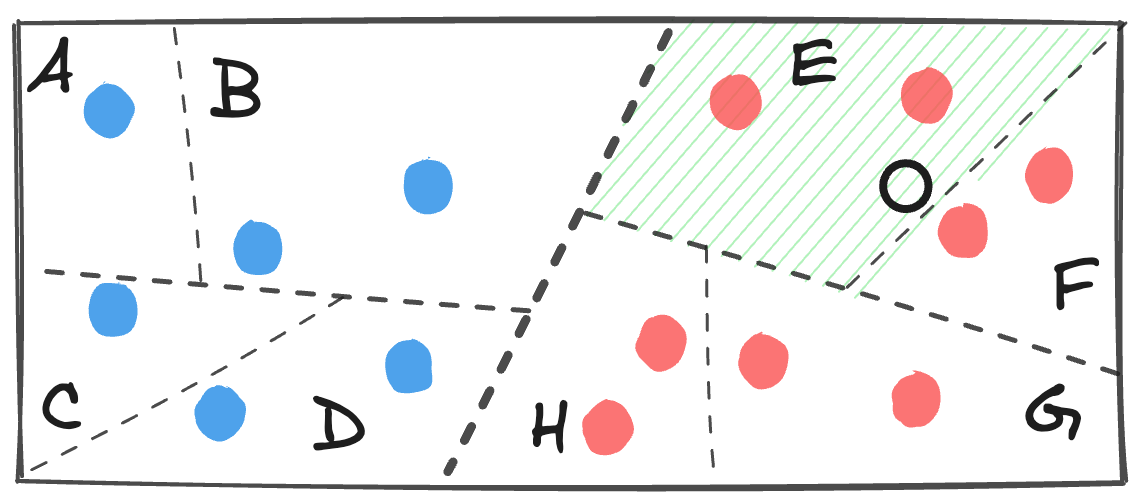
\includegraphics[width=0.47\linewidth]{figures/branch-and-bound-hard-and-fast.png}
    }
    \subfloat[]{
        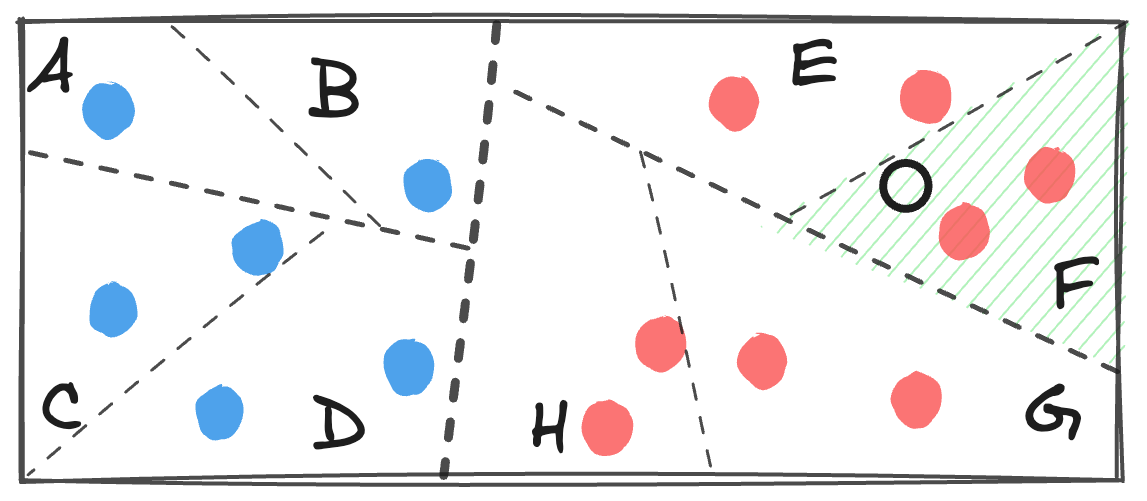
\includegraphics[width=0.47\linewidth]{figures/branch-and-bound-randomized.png}
    }
    \caption{Randomized construction of $k$-d Trees for a fixed collection of vectors (filled circles).
    Decision boundaries take random directions
    and are planted at a randomly-chosen point near the median. Repeating this procedure
    results in multiple ``index'' structures of the vector collection. Performing a ``defeatist'' search
    repeatedly for a given query (the empty circles) then leads to a higher probability of success.}
    \label{figure:branch-and-bound:randomized}
\end{figure}

Would the situation be different if tree construction was a randomized algorithm?
We could, for instance, let a random subset of the data points that are close to
each decision boundary fall into both ``left'' and ``right'' sub-regions as we split an internal node.
As another example, we could place the decision boundaries at randomly chosen points
close to the median, and have them take a randomly chosen direction.
We illustrate the latter in Figure~\ref{figure:branch-and-bound:randomized}.

\begin{svgraybox}
Such randomized decisions mean that, every time we construct a $k$-d Tree, we would obtain a different
index of the data. Furthermore, by building a forest of randomized $k$-d Trees and repeating
the defeatist search algorithm, we may be able to lower the failure probability!
\end{svgraybox}

These, as we will learn in this section, are indeed successful ideas that have
been extensively explored in the literature~\citep{liu2004SpillTree,ram2019revisiting_kdtree,dasgupta2015rptrees}.

\subsection{Randomized Partition Trees}

Recall that a decision boundary in a $k$-d Tree is an axis-aligned hyperplane that is placed at the median point
of the projection of data points onto a coordinate axis.
Consider the following adjustment to that procedure, due originally to~\cite{liu2004SpillTree}
and further refined by~\cite{dasgupta2015rptrees}.
Every time a node whose region is $\mathcal{R}$ is to be split, we first draw a \emph{random direction}
$u$ by sampling a vector from the $d$-dimensional unit sphere, and a scalar $\beta \in [1/4, 3/4]$ uniformly at random.
We then project all data points that are in $\mathcal{R}$ onto $u$,
and obtain the $\beta$-fractile of the projections, $\theta$. $u$ together with $\theta$ form the decision
boundary. We then proceed as before to partition the data points in $\mathcal{R}$, by following the rule
$\langle u, v \rangle \leq \theta$ for every data point $v \in \mathcal{R}$.
A node turns into a leaf if it contains a maximum of $m_\circ$ vectors.

The procedure above gives us what~\cite{dasgupta2015rptrees} call a \emph{Randomized Partition} (RP) Tree.
You have already seen a visual demonstration of two RP Trees in Figure~\ref{figure:branch-and-bound:randomized}.
Notice that, by requiring $u$ to be a standard basis vector, fixing one $u$ per each level of the tree,
and letting $\beta=0.5$, we reduce an RP Tree to the original $k$-d Tree.

What is the probability that a defeatist search over a single RP Tree fails to return the correct nearest neighbor?
\cite{dasgupta2015rptrees} proved that, that probability is related to the following potential function:
\begin{equation}
    \label{equation:branch-and-bound:randomized:potential}
    \Phi(q, \mathcal{X}) = \frac{1}{m} \sum_{i=1}^{m}
    \frac{\lVert q - x^{(\pi_1)} \rVert_2}{\lVert q - x^{(\pi_i)} \rVert_2},
\end{equation}
where $m = \lvert \mathcal{X} \rvert$, $\pi_1$ through $\pi_m$ are indices that
sort data points by increasing distance to the query point $q$, so that $x^{(\pi_1)}$
is the closest data point to $q$.

\begin{svgraybox}
Notice that, a value of $\Phi$ that is close to $1$ implies that nearly
all data points are at the same distance from $q$. In that case, as we saw in Chapter~\ref{chapter:instability},
NN becomes unstable and approximate top-$k$ retrieval becomes meaningless.
When $\Phi$ is closer to $0$, on the other hand, the optimal vector is well-separated
from the rest of the collection.

Intuitively then, $\Phi$ is reflective of the difficulty or stability of the NN problem for a given query point.
It makes sense then, that the probability of failure for $q$ is related to this notion of difficulty
of NN search: intuitively, when the nearest neighbor is far from other vectors, a defeatist search is more likely
to yield the correct solution.
\end{svgraybox}

\subsubsection{A Potential Function to Quantify the Difficulty of NN Search}

Before we state the relationship between the failure probability and the potential function above more concretely,
let us take a detour and understand where the expression for $\Phi$ comes from. All the arguments that we are about
to make, including the lemmas and theorems, come directly from~\cite{dasgupta2015rptrees}, 
though we repeat them here using our adopted notation for completeness. We also present an
expanded proof of the formal results which follows the original proofs but elaborates on some of the steps.

\medskip

Let us start with a simplified setup where $\mathcal{X}$ consists of just two vectors $x$ and $y$.
Suppose that for a query point $q$, $\lVert q - x \rVert_2 \leq \lVert q - y \rVert_2$.
It turns out that, if we chose a random direction $u$ and projected $x$ and $y$ onto it,
then the probability that the projection of $y$ onto $u$ lands somewhere in between the projections of
$q$ and $x$ onto $u$ is a function of the potential function of Equation~(\ref{equation:branch-and-bound:randomized:potential}).
The following lemma formalizes this relationship.

\begin{lemma}
    \label{lemma:branch-and-bound:randomized:two-points}
    Suppose $q, x, y \in \mathbb{R}^d$ and $\lVert q - x \rVert_2 \leq \lVert q - y \rVert_2$.
    Let $U \in \mathbb{S}^{d-1}$ be a random direction and define
    $\overset{\angle}{v} = \langle U, v \rangle$.
    The probability that $\overset{\angle}{y}$ is between $\overset{\angle}{q}$ and $\overset{\angle}{x}$
    is:
    \begin{align*}
        \probability\big[
            \big( \overset{\angle}{q} \leq \overset{\angle}{y} \leq \overset{\angle}{x} \big) \lor
            \big( \overset{\angle}{x} \leq \overset{\angle}{y} \leq \overset{\angle}{q} \big) \big] &= \\
        \frac{1}{\pi} \arcsin \Biggl( 2 \Phi(q, \{ x, y\})
            & \sqrt{1 - \Big(
                \frac{\langle q - x, y - x \rangle}{\lVert q - x \rVert_2 \lVert y - x \rVert_2}
            \Big)^2}
        \Biggr).
    \end{align*}
\end{lemma}
\begin{proof}
Assume, without loss of generality, that $U$ is sampled from a $d$-dimensional standard Normal distribution: $U \sim \mathcal{N}(\mathbf{0}, I_d)$.
That assumption is inconsequential because normalizing $U$ by its $L_2$ norm gives a vector that lies on $\mathbb{S}^{d-1}$ as required.
But because the norm of $U$ does not affect the argument we need not explicitly perform the normalization.

Suppose further that we translate all vectors by $q$,
and redefine $q \triangleq \mathbf{0}$, $x \triangleq x - q$, and $y \triangleq y - q$.
We then rotate the vectors so that $x = \lVert x \rVert_2 e_1$, where $e_1$ is the first standard basis vector.
Neither the translation nor the rotation affects pairwise distances, and as such, no generality is lost due to these transformations.

Given this arrangement of vectors, it will be convenient to write $U = (U_1, U_{\setminus 1})$ and $y = (y_1, y_{\setminus 1})$
so as to make explicit the first coordinate of each vector (denoted by subscript $1$)
and the remaining coordinates (denoted by subscript $\setminus 1$).

It is safe to assume that $y_{\setminus 1} \neq \mathbf{0}$. The reason is that, if that were not the case,
the two vectors $x$ and $y$ have an intrinsic dimensionality of $1$ and are thus on a line.
In that case, no matter which direction $U$ we choose, $\overset{\angle}{y}$ will not fall between
$\overset{\angle}{x}$ and $\overset{\angle}{q} = \mathbf{0}$.

We can now write the probability of the event of interest as follows:
\begin{align*}
    \probability&\Big[
        \underbrace{
            \big( \overset{\angle}{q} \leq \overset{\angle}{y} \leq \overset{\angle}{x} \big) \lor
            \big( \overset{\angle}{x} \leq \overset{\angle}{y} \leq \overset{\angle}{q} \big) }_{E}\Big] = \\
    &\probability\Big[
            \big( 0 \leq \langle U, y \rangle \leq \lVert x \rVert_2 U_1 \big) \lor
            \big( \lVert x \rVert_2 U_1 \leq \langle U, y \rangle \leq 0 \big) \Big].
\end{align*}
By expanding $\langle U, y \rangle = y_1 U_1 + \langle U_{\setminus 1}, y_{\setminus 1} \rangle$, it becomes clear that the expression
above measures the probability that $\langle U_{\setminus 1}, y_{\setminus 1} \rangle$ falls in the interval
$\big(-y_1 \lvert U_1 \rvert, (\lVert x \rVert_2 - y_1)\lvert U_1 \rvert \big)$ when $U_1 \geq 0$ or
$\big(-(\lVert x \rVert_2 - y_1) \lvert U_1 \rvert, y_1 \lvert U_1 \rvert\big)$ otherwise.
As such $\probability[E]$ can be rewritten as follows:
\begin{align*}
    \probability[E] &=
    \probability\Big[
            -y_1 \lvert U_1 \rvert \leq \langle U_{\setminus 1}, y_{\setminus 1} \rangle \leq (\lVert x \rVert_2 - y_1)\lvert U_1 \rvert \;\big|\; U_1 \geq 0 \Big] \probability\big[ U_1 \geq 0 \big] \\
    &+ \probability\Big[-(\lVert x \rVert_2 - y_1)\lvert U_1 \rvert \leq \langle U_{\setminus 1}, y_{\setminus 1} \rangle \leq y_1 \lvert U_1 \rvert \;\big|\; U_1 < 0 \Big] \probability\big[ U_1 < 0 \big].
\end{align*}
First, note that $U_1$ is independent of $U_{\setminus 1}$ given that they are sampled from $\mathcal{N}(\mathbf{0}, I_d)$.
Second, observe that $\langle U_{\setminus 1}, y_{\setminus 1} \rangle$ is distributed as $\mathcal{N}(\mathbf{0}, \lVert y_{\setminus 1} \rVert_2^2)$,
which is symmetric, so that the two intervals have the same probability mass.
These two observations simplify the expression above, so that $\probability[E]$ becomes:
\begin{align*}
    \probability[ E ] &= \probability\Big[ -y_1 \lvert U_1 \rvert \leq \langle U_{\setminus 1}, y_{\setminus 1} \rangle \leq (\lVert x \rVert_2 - y_1)\lvert U_1 \rvert \Big] \\
    &= \probability\Big[ -y_1 \lvert Z \rvert \leq \lVert y_{\setminus 1} \rVert_2 Z^\prime \leq (\lVert x \rVert_2 - y_1)\lvert Z \rvert \Big] \\
    &= \probability\Bigg[ \frac{\lvert Z' \rvert}{\lvert Z \rvert} \in \Big( -\frac{y_1}{\lVert y_{\setminus 1} \rVert_2}, \frac{\lVert x \rVert_2 - y_1}{\lVert y_{\setminus 1} \rVert_2} \Big) \Bigg],
\end{align*}
where $Z$ and $Z^\prime$ are independent random variables drawn from $\mathcal{N}(0, 1)$.

Using the fact that the ratio of two independent Gaussian random variables follows a standard Cauchy distribution,
we can calculate $\probability[ E ]$ as follows:
\begin{align*}
    \probability[ E ] &= \int_{-y_1/\lVert y_{\setminus 1} \rVert_2}^{\big(\lVert x \rVert_2 - y_1\big)/\lVert y_{\setminus 1} \rVert_2} \frac{d \omega}{\pi (1 + \omega^2)} \\
    &= \frac{1}{\pi} \Bigg[ \arctan\Big( \frac{\lVert x \rVert_2 - y_1}{\lVert y_{\setminus 1} \rVert_2} \Big) - \arctan \Big( -\frac{y_1}{\lVert y_{\setminus 1} \rVert_2} \Big) \Bigg] \\
    &= \frac{1}{\pi} \arctan\Bigg( \frac{\lVert x \rVert_2 \lVert y_{\setminus 1} \rVert_2}{\lVert y \rVert_2^2 - y_1 \lVert x \rVert_2} \Bigg) \\
    &= \frac{1}{\pi} \arcsin\Bigg( \frac{\lVert x \rVert_2}{\lVert y \rVert_2} \sqrt{\frac{\lVert y \rVert_2^2 - y_1^2}{\lVert y \rVert_2^2 - 2y_1 \lVert x \rVert_2 + \lVert x \rVert_2^2}} \Bigg).
\end{align*}
In the third equality, we used the fact that $\arctan a + \arctan b = \arctan (a + b)/(1 - ab)$, and in the fourth equality
we used the identity $\arctan a = \arcsin a / \sqrt{1 + a^2}$. Substituting $y_1 = \langle y, x \rangle / \lVert x \rVert_2$
and noting that $x$ and $y$ have been shifted by $q$ completes the proof.
\end{proof}

\begin{corollary}
\label{lemma:branch-and-bound:randomized:two-points-corollary}
    In the same configuration as in Lemma~\ref{lemma:branch-and-bound:randomized:two-points}:
    \begin{align*}
        \frac{2}{\pi} \Phi(q, \{ x, y\})
            & \sqrt{1 - \Big(
                \frac{\langle q - x, y - x \rangle}{\lVert q - x \rVert_2 \lVert y - x \rVert_2}
            \Big)^2} \leq& \\
        &\probability\Big[
            \big( \overset{\angle}{q} \leq \overset{\angle}{y} \leq \overset{\angle}{x} \big) \lor
            \big( \overset{\angle}{x} \leq \overset{\angle}{y} \leq \overset{\angle}{q} \big) \Big] \leq 
            \Phi(q, \{ x, y\})
    \end{align*}
\end{corollary}
\begin{proof}
Applying the inequality $\theta \geq \sin \theta \geq 2 \theta/\pi$ for $0 \leq \theta \leq \pi/2$ to Lemma~\ref{lemma:branch-and-bound:randomized:two-points}
implies the claim.
\end{proof}

Now that we have examined the case of $\mathcal{X} = \{ x, y\}$, it is easy to extend
the result to a configuration of $m$ vectors.

\begin{theorem}
    \label{theorem:branch-and-bound:randomized:m-points}
    Suppose $q \in \mathbb{R}^d$, $\mathcal{X} \subset \mathbb{R}^d$ is a set of $m$ vectors,
    and $x^\ast \in \mathcal{X}$ the nearest neighbor of $q$.
    Let $U \in \mathbb{S}^{d-1}$ be a random direction, define $\overset{\angle}{v} = \langle U, v \rangle$,
    and let $\overset{\angle}{\mathcal{X}} = \{ \overset{\angle}{x} \;|\; x \in \mathcal{X} \}$.
    Then:
    \begin{equation*}
        \mathbb{E}_{U} \big[ \textit{fraction of $\overset{\angle}{\mathcal{X}}$ that is between
        $\overset{\angle}{q}$ and $\overset{\angle}{x^\ast}$} \big] \leq \frac{1}{2} \Phi(q, \mathcal{X}).
    \end{equation*}
\end{theorem}
\begin{proof}
    Let $\pi_1$ through $\pi_m$ be indices that order the elements of $\mathcal{X}$ by increasing distance to $q$,
    so that $x^\ast = x^{(\pi_1)}$. Denote by $Z_i$ the event that $\langle U, x^{(\pi_i)} \rangle$ falls between $\overset{\angle}{x^\ast}$
    and $\overset{\angle}{q}$. By Corollary~\ref{lemma:branch-and-bound:randomized:two-points-corollary}:
    \begin{equation*}
        \probability[Z_i] \leq \frac{1}{2} \frac{\lVert q - x^{(\pi_1)} \rVert_2}{\lVert q - x^{(\pi_i)} \rVert_2}.
    \end{equation*}
    We can now write the expectation of interest as follows:
    \begin{equation*}
        \sum_{i=2}^{m} \frac{1}{m} \probability[ Z_i ] \leq \frac{1}{2} \Phi(q, \mathcal{X}).
    \end{equation*}
\end{proof}.

\begin{corollary}
    \label{corollary:branch-and-bound:randomized:m-points}
    Under the assumptions of Theorem~\ref{theorem:branch-and-bound:randomized:m-points}, for any $\alpha \in (0, 1)$
    and any $s$-subset $S$ of $\mathcal{X}$ that contains $x^\ast$:
    \begin{equation*}
        \probability\big[ \textit{at least $\alpha$ fraction of $\overset{\angle}{S}$ is between
        $\overset{\angle}{q}$ and $\overset{\angle}{x^\ast}$} \big] \leq \frac{1}{2\alpha} \Phi_s(q, \mathcal{X}),
    \end{equation*}
    where:
    \begin{equation*}
        \Phi_s(q, \mathcal{X}) = \frac{1}{s} \sum_{i=1}^{s}
    \frac{\lVert q - x^{(\pi_1)} \rVert_2}{\lVert q - x^{(\pi_i)} \rVert_2},
    \end{equation*}
    and $\pi_1$ through $\pi_s$ are indices of the $s$ vectors in $\mathcal{X}$ that are closest to $q$, ordered
    by increasing distance.
\end{corollary}
\begin{proof}
    Apply Theorem~\ref{theorem:branch-and-bound:randomized:m-points} to the set $S$ to obtain:
    \begin{equation*}
        \mathbb{E}\big[ \textit{fraction of $\overset{\angle}{S}$ that is between
        $\overset{\angle}{q}$ and $\overset{\angle}{x^\ast}$} \big] \leq \frac{1}{2} \Phi(q, S) \leq \frac{1}{2} \Phi_s(q, \mathcal{X}).
    \end{equation*}
    Using Markov's inequality (i.e., $\probability[Z > \alpha] \leq \mathbb{E}[Z]/\alpha$) completes the proof.
\end{proof}

The above is where the potential function of Equation~(\ref{equation:branch-and-bound:randomized:potential}) first emerges
in its complete form for an arbitrary collection of vectors and its subsets.
As we see, $\Phi$ bounds the expected number of vectors whose projection onto
a random direction $U$ falls between a query point and its nearest neighbor.

\begin{svgraybox}
The reason this expected value is important (which subsequently justifies the importance of
$\Phi$) has to do with the fact that decision boundaries are planted at some $\beta$-fractile point of
the projections. As such, a bound on the number of points that fall between
$q$ and its nearest neighbor serves as a tool to bound the odds that the decision boundary may separate $q$ from
its nearest neighbor, which is the failure mode we wish to quantify.
\end{svgraybox}

\subsubsection{Probability of Failure}
We are now ready to use Theorem~\ref{theorem:branch-and-bound:randomized:m-points} and
Corollary~\ref{corollary:branch-and-bound:randomized:m-points} to derive the failure probability
of the defeatist search over an RP Tree.
To that end, notice that, the path from the root to a leaf is a sequence of $\log_{1/\beta} (m/m_\circ) $
independent decisions that involve randomly projected data points. So if we were able to bound the failure probability
of a single node, we can apply the union bound and obtain a bound on the failure probability of the tree.
That is the intuition that leads to the following result.

\begin{theorem}
    The probability that an RP Tree built for collection $\mathcal{X}$ of $m$ vectors fails to find the nearest neighbor
    of a query $q$ is at most:
    \begin{equation*}
        \sum_{l = 0}^{\ell} \Phi_{\beta^l m} \ln \frac{2e}{\Phi_{\beta^l m}},
    \end{equation*}
    with $\beta = 3/4$ and $\ell = \log_{1/\beta} \big( m / m_\circ \big)$, and where we use the shorthand
    $\Phi_s$ for $\Phi_s(q, \mathcal{X})$.
\end{theorem}
\begin{proof}
    Consider an internal node of the RP Tree that contains $q$ and $s$ data points including $x^\ast$, the nearest neighbor of $q$.
    If the decision boundary at this node separates $q$ from $x^\ast$, then the defeatist search will fail.
    We therefore seek to quantify the probability of that event.

    Denote by $F$ the fraction of the $s$ vectors that, once projected onto the random direction $U$ associated with the node,
    fall between $q$ and $x^\ast$. Recall that, the split threshold associated with the node is drawn uniformly from an interval
    of mass $1/2$. As such, the probability that $q$ is separated from $x^\ast$ is at most
    $F/(1/2)$. By integrating over $F$, we obtain:
    \begin{align*}
        \probability\big[ \textit{$q$ is separated from $x^\ast$} \big] &\leq \int_0^1 \probability\big[ F = f\big] \frac{f}{1/2} df \\
        &= 2 \int_0^1 \probability\big[ F > f \big] df \\
        &\leq 2 \int_0^1 \min \Big( 1, \frac{\Phi_s}{2f} \Big) df \\
        &= 2 \int_0^{\Phi_s / 2} df + 2 \int_{\Phi_s / 2}^ 1 \frac{\Phi_s}{2f} df \\
        &= \Phi_s \ln \frac{2e}{\Phi_s}.
    \end{align*}
    The first equality uses the definition of expectation for a positive random variable,
    while the second inequality uses Corollary~\ref{corollary:branch-and-bound:randomized:m-points}.
    Applying the union bound to a path from root to leaf,
    and noting that the size of the collection that falls into each node
    drops geometrically per level by a factor of at least $3/4$ completes the proof.
\end{proof}

We are thus able to express the failure probability as a function of $\Phi$,
a quantity that is defined for a particular $q$ and a concrete collection of vectors.
If we have a model of the data distribution, it may be possible to
state more general bounds by bounding $\Phi$ itself.~\cite{dasgupta2015rptrees}
demonstrate examples of this for two practical data distributions.
Let us review one such example here.

\subsubsection{Data Drawn from a Doubling Measure}
\label{section:branch-and-bound:doubling-measure}
Throughout our analysis of $k$-d Trees in Section~\ref{section:branch-and-bound:kd-tree},
we considered the case where data points are uniformly distributed in $\mathbb{R}^d$.
As we argued in Chapter~\ref{chapter:intrinsic-dimensionality}, in many practical situations,
however, even though vectors are represented in $\mathbb{R}^d$,
they actually lie in some low-dimensional manifold with \emph{intrinsic dimension}
$d_\circ$ where $d_\circ \ll d$.
This happens, for example, when data points are drawn from a \emph{doubling measure}
with low dimension as defined in Definition~\ref{definition:doubling-measure}.

\begin{svgraybox}
\cite{dasgupta2015rptrees} prove that, if a collection of $m$ vectors is sampled
from a doubling measure with dimension $d_\circ$,
then $\Phi$ can be bounded from above roughly by $(1/m)^{1/d_\circ}$. The following
theorem presents their claim.
\end{svgraybox}

\begin{theorem}
    Suppose a collection $\mathcal{X}$ of $m$ vectors is drawn from $\mu$, a continuous, doubling measure
    on $\mathbb{R}^d$ with dimension $d_\circ \geq 2$. For an arbitrary $\delta \in (0, 1/2)$,
    with probability at least $1 - 3\delta$, for all $2 \leq s \leq m$:
    \begin{equation*}
        \Phi_s(q, \mathcal{X}) \leq 6 \Bigg( \frac{2}{s} \ln \frac{1}{\delta} \Bigg)^{1/d_\circ}.
    \end{equation*}
\end{theorem}

Using the result above,~\cite{dasgupta2015rptrees} go on to prove that,
under the same conditions, with probability at least $1 - 3\delta$,
the failure probability of an RP Tree is bounded above by:
\begin{equation*}
    c_\circ (d_\circ + \ln m_\circ) \Bigg( \frac{8 \max (1, \ln 1/\delta)}{m_\circ} \Bigg)^{1/d_\circ},
\end{equation*}
where $c_\circ$ is an absolute constant, and $m_\circ \geq c_\circ 3^{d_\circ} \max (1, \ln 1/\delta)$.

\begin{svgraybox}
The results above tell us that, so long as the space has a small intrinsic
dimension, we can make the probability of failing to find the optimal solution
arbitrarily small.
\end{svgraybox}

\subsection{Spill Trees}
The Spill Tree~\citep{liu2004SpillTree} is another randomized variant of the $k$-d Tree.
The algorithm to construct a Spill Tree comes with a hyperparameter $\alpha \in [0, 1/2]$
that is typically a small constant closer to $0$.
Given an $\alpha$, the Spill Tree modifies the tree construction algorithm of the $k$-d Tree as follows.
When splitting a node whose region is $\mathcal{R}$, we first project all vectors contained
in $\mathcal{R}$ onto a random direction $U$, then find the median of the resulting distribution.
However, instead of \emph{partitioning} the vectors based on which side of the median they are on,
the algorithm forms two overlapping sets. The ``left'' set contains all vectors in $\mathcal{R}$
whose projection onto $U$ is smaller than the $(1/2 + \alpha)$-fractile point of the distribution,
while the ``right'' set consists of those that fall to the right of the $(1/2 - \alpha)$-fractile point.
As before, a node becomes a leaf when it has a maximum of $m_\circ$ vectors.

\begin{figure}[t]
    \centering
    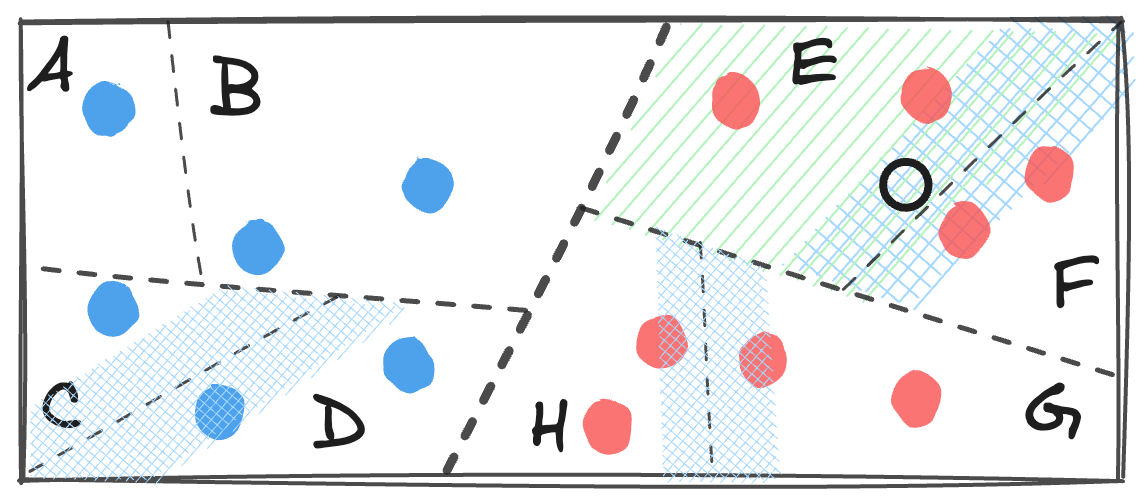
\includegraphics[width=0.6\linewidth]{figures/branch-and-bound-spill-tree.png}
    \caption{Defeatist search over a Spill Tree. In a Spill Tree, vectors that are
    close to the decision boundary are, in effect, duplicated, with their copy ``spilling'' over
    to the other side of the boundary. This is depicted for a few example regions
    as the blue shaded area that straddles the decision boundary: vectors that fall into the shaded
    area belong to neighboring regions. For example, regions $G$ and $H$ share two vectors.
    As such, a defeatist search for the example query (the empty circle) looks through not just the region
    $E$ but its extended region that overlaps with $F$.}
    \label{figure:branch-and-bound:spill-tree}
\end{figure}

During search, the algorithm performs a defeatist search by routing the query point $q$
based on a comparison of its projection onto the random direction associated with each node,
and the \emph{median} point. It is clear that with this strategy, if the nearest neighbor
of $q$ is close to the decision boundary of a node, we do not increase the likelihood of
failure whether we route $q$ to the left child or to the right one. Figure~\ref{figure:branch-and-bound:spill-tree}
shows an example of the defeatist search over a Spill Tree.

\subsubsection{Space Overhead}
One obvious downside of the Spill Tree is that a single data point
may end up in multiple leaf nodes, which increases the space complexity.
We can quantify that by noting that the depth of the tree on a collection of $m$ vectors
is at most $\log_{1/(1/2 + \alpha)} (m/m_\circ)$, so that the total number of vectors in all leaves
is:
\begin{equation*}
    m_\circ 2^{\log_{1/(1/2 + \alpha)} (m/m_\circ)} = m_\circ \big( \frac{m}{m_\circ} \big)^{\log_{1/(1/2 + \alpha)} 2} =
    m_\circ \big( \frac{m}{m_\circ} \big)^{1/(1 - \log(1 + 2\alpha))}.
\end{equation*}
As such, the space complexity of a Spill Tree is $\mathcal{O}(m^{1/(1 - \log(1 + 2 \alpha))})$.

\subsubsection{Probability of Failure}
The defeatist search over a Spill Tree fails to return the nearest neighbor $x^\ast$
if the following event takes place at any of the nodes that contains $q$ and $x^\ast$.
That is the event where the projections of $q$ and $x^\ast$ are separated by the median \emph{and}
where the projection of $x^\ast$ is separated from the median by at least $\alpha$-fraction of the vectors.
That event happens when the projections of $q$ and $x^\ast$ are separated by
at least $\alpha$-fraction of the vectors in some node along the path.

The probability of the event above can be bounded by Corollary~\ref{corollary:branch-and-bound:randomized:m-points}.
By applying the union bound to a root-to-leaf path, and noting that the size of the collection
reduces at each level by a factor of at least $1/2 + \alpha$, we obtain the following result:

\begin{theorem}
    The probability that a Spill Tree built for collection $\mathcal{X}$ of $m$ vectors fails to find the nearest neighbor
    of a query $q$ is at most:
    \begin{equation*}
        \sum_{l = 0}^{\ell} \frac{1}{2\alpha} \Phi_{\beta^l m}(q, \mathcal{X}),
    \end{equation*}
    with $\beta = 1/2 + \alpha$ and $\ell = \log_{1/\beta} \big( m / m_\circ \big)$.
\end{theorem}

\section{Cover Trees}
The branch-and-bound algorithms we have reviewed thus far divide a
collection recursively into exactly two sub-collections, using a 
hyperplane as a decision boundary. Some also have a certification process
that involves backtracking from a leaf node whose region contains a query
to the root node. As we noted in Section~\ref{section:branch-and-bound:intuition},
however, none of these choices is absolutely necessary. In fact,
branching and bounding can be done entirely differently. We review
in this section a popular example that deviates from that pattern,
a data structure known as the Cover Tree~\citep{covertrees}.

It is more intuitive to describe the Cover Tree, as well as the construction
and search algorithms over it, in the abstract first. This is
what~\cite{covertrees} call the \emph{implicit} representation.
Let us first describe its structure, then review its properties
and explain the relevant algorithms,
and only then discuss how the abstract tree can be implemented concretely.

\subsection{The Abstract Cover Tree and its Properties}

The abstract Cover Tree is a tree structure with infinite depth
that is defined for a proper metric $\delta(\cdot, \cdot)$.
Each level of the tree is numbered by an integer that starts
from $\infty$ at the level of the root node and decrements, to $-\infty$,
at each subsequent level.
Each node represents a single data point.
If we denote the collection of nodes on level $\ell$ by $C_\ell$,
then $C_\ell$ is a \emph{set}, in the sense that the
data points represented by those nodes are distinct.
But $C_\ell \subset C_{\ell - 1}$, so that once a node
appears in level $\ell$, it necessarily appears in levels $(\ell - 1)$
onward. That implies that, in the abstract Cover Tree, $C_\infty$ contains
a single data point, and $C_{-\infty} = \mathcal{X}$ is the entire collection.

\begin{figure}[t]
    \centering
    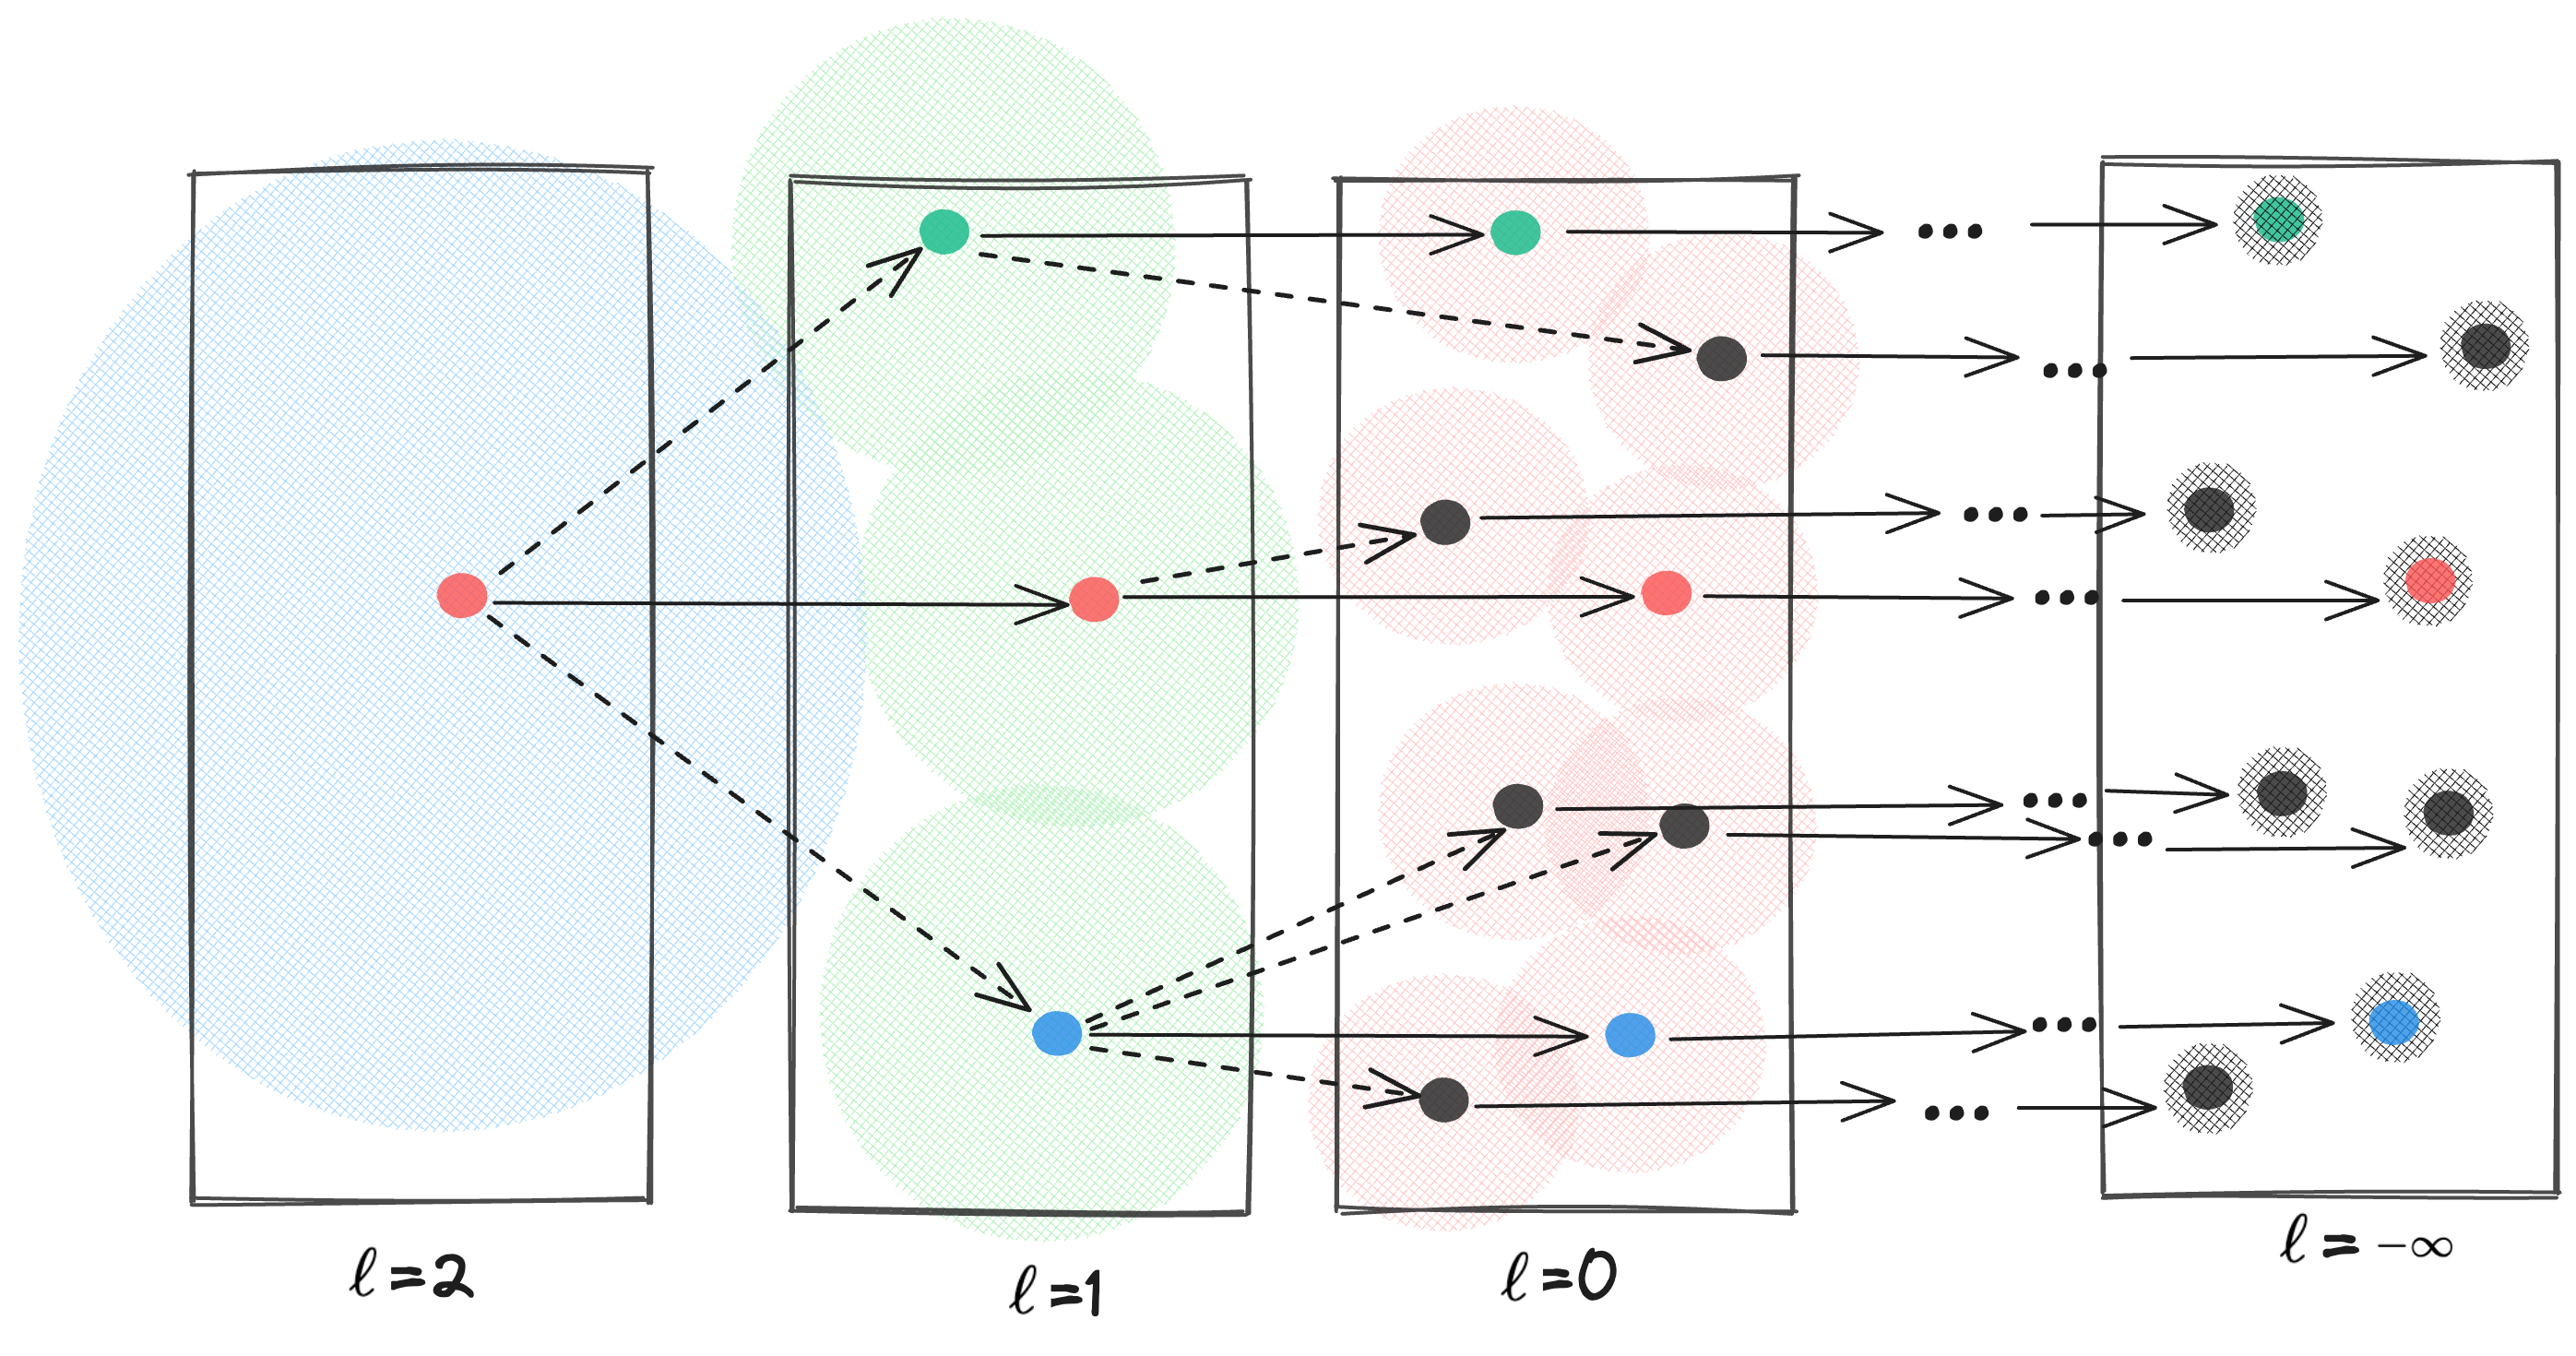
\includegraphics[width=0.7\linewidth]{figures/branch-and-bound-abstract-cover-tree.png}
    \caption{Illustration of the abstract Cover Tree for a collection of $8$ vectors.
    Nodes on level $\ell$ of the tree are separated by at least $2^\ell$ by the separation invariant.
    Nodes on level $\ell$ cover nodes on level $(\ell - 1)$ with a ball of radius
    at most $2^\ell$ by the covering invariant.
    Once a node appears in the tree, it will appear on all subsequent
    levels as its own child (solid arrows), by the nesting invariant.}
    \label{figure:branch-and-bound:abstract-cover-tree}
\end{figure}

This structure, which is illustrated in Figure~\ref{figure:branch-and-bound:abstract-cover-tree}
for an example collection of vectors, obeys three invariants. That is, all algorithms
that construct the tree or manipulate it in any way must guarantee
that the three properties are not violated. These invariants are:
\begin{itemize}
    \item \textbf{Nesting}: As we noted, $C_\ell \subset C_{\ell - 1}$.
    \item \textbf{Covering}: For every node $u \in C_{\ell - 1}$
    there is a node $v \in C_\ell$ such that $\delta(u, v) < 2^\ell$.
    In other words, every node in the next level $(\ell - 1)$ of the tree is ``covered''
    by an open ball of radius $2^\ell$ around a node in the current level, $\ell$.
    \item \textbf{Separation}: All nodes on the same level $\ell$ are separated by
    a distance of at least $2^\ell$. Formally, if $u, v \in C_\ell$, then $\delta(u, v) > 2^\ell$.
\end{itemize}

\subsection{The Search Algorithm}
We have seen what a Cover Tree looks like and what properties it is guaranteed to maintain.
Given this structure, how do we find the nearest neighbor of a query point?
That turns out to be a fairly simple algorithm as shown in Algorithm~\ref{algorithm:branch-and-bound:cover-tree:nn-search}.

\begin{algorithm}[!t]
\SetAlgoLined
{\bf Input: }{Cover Tree with metric $\delta(\cdot, \cdot)$; query point $q$.}\\
\KwResult{Exact NN of $q$.}

\begin{algorithmic}[1]

\STATE $Q_\infty \leftarrow C_\infty$ \Comment*[l]{\footnotesize $C_\ell$ is the set of nodes on level $\ell$}

\FOR{$\ell$ from $\infty$ to $-\infty$} \label{algorithm:branch-and-bound:cover-tree:nn-search:loop}
    \STATE $Q \leftarrow \{ \textsc{Children}(v) \;|\; v \in Q_\ell \}$ \Comment*[l]{\footnotesize \textsc{Children}$(\cdot)$ returns the children of its argument.}
    \STATE $Q_{\ell - 1} \leftarrow \{ u \;|\; \delta(q, u) \leq \delta(q, Q) + 2^\ell \}$ \Comment*[l]{\footnotesize $\delta(u, S) \triangleq \min_{v \in S} \delta(u, v)$.}\label{algorithm:branch-and-bound:cover-tree:nn-search:pruning}
\ENDFOR

\RETURN $\argmin_{u \in Q_{-\infty}} \delta(q, u)$ \label{algorithm:branch-and-bound:cover-tree:nn-search:return}
\end{algorithmic}
\caption{Nearest Neighbor search over a Cover Tree.}
\label{algorithm:branch-and-bound:cover-tree:nn-search}
\end{algorithm}

Algorithm~\ref{algorithm:branch-and-bound:cover-tree:nn-search} always maintains a current
set of candidates in $Q_\ell$ as it visits level $\ell$ of the tree. In each iteration of the
loop on Line~\ref{algorithm:branch-and-bound:cover-tree:nn-search:loop}, it creates a temporary
set---denoted by $Q$---by collecting the children of all nodes in $Q_\ell$. It then prunes the nodes
in $Q$ based on the condition on Line~\ref{algorithm:branch-and-bound:cover-tree:nn-search:pruning}.
Eventually, the algorithm returns the exact nearest neighbor of query $q$ by
performing exhaustive search over the nodes in $Q_{-\infty}$.

Let us understand why the algorithm is correct. In a way, it is enough to argue that
the pruning condition on Line~\ref{algorithm:branch-and-bound:cover-tree:nn-search:pruning}
never discards an ancestor of the nearest neighbor. If that were the case, we are done
proving the correctness of the algorithm: $Q_{-\infty}$ is guaranteed to have the nearest neighbor,
at which point we will find it on Line~\ref{algorithm:branch-and-bound:cover-tree:nn-search:return}.

The fact that Algorithm~\ref{algorithm:branch-and-bound:cover-tree:nn-search} never prunes
the ancestor of the solution is easy to establish.
To see how, consider the distance between $u \in C_{\ell-1}$ and any of its descendants, $v$.
The distance between the two vectors is bounded as follows:
$\delta(u, v) \leq \sum_{l = \ell - 1}^{-\infty} 2^l = 2^\ell$.
Furthermore, because $\delta$ is proper, by triangle inequality, we know
that: $\delta(q, u^\ast) \leq \delta(q, Q) + \delta(Q, u^\ast)$, where
$u^\ast$ is the solution and a descendant of $u \in C_{\ell - 1}$.
As such, any candidate whose distance is greater than
$\delta(q, Q) + \delta(Q, u^\ast) \leq \delta(q, Q) + 2^\ell$ can be safely
pruned.

\bigskip

The search algorithm has an $\epsilon$-approximate variant too.
To obtain a solution that is at most $(1 + \epsilon) \delta(q, u^\ast)$
away from $q$, assuming $u^\ast$ is the optimal solution, we need 
only to change the termination condition on Line~\ref{algorithm:branch-and-bound:cover-tree:nn-search:loop},
by exiting the loop as soon as $\delta(q, Q_{\ell}) \geq 2^{\ell + 1} (1 + 1/\epsilon)$.
Let us explain why the resulting algorithm is correct.

Suppose that the algorithm terminates early when it reaches level $\ell$.
That means that $2^{\ell + 1} (1 + 1/\epsilon) \leq \delta(q, Q_\ell)$.
We have already seen that $\delta(q, Q_\ell) \leq 2^{\ell + 1}$, and by triangle
inequality, that $\delta(q, Q_\ell) \leq \delta(q, u^\ast) + 2^{\ell + 1}$.
So we have bounded $\delta(q, Q_\ell)$ from below and above, resulting
in the following inequality:
\begin{equation*}
    2^{\ell + 1} \Big( 1 + \frac{1}{\epsilon} \Big) \leq \delta(q, u^\ast) + 
    2^{\ell + 1} \implies 2^{\ell + 1} \leq \epsilon \delta(q, u^\ast).
\end{equation*}
Putting all that together, we have shown that $\delta(q, Q_\ell) \leq (1 + \epsilon) \delta(q, u^\ast)$,
so that Line~\ref{algorithm:branch-and-bound:cover-tree:nn-search:return} returns an $\epsilon$-approximate
solution.

\subsection{The Construction Algorithm}
Inserting a single vector into the Cover Tree ``index'' is a procedure
that is similar to the search algorithm but is better conceptualized recursively,
as shown in Algorithm~\ref{algorithm:branch-and-bound:cover-tree:insertion}.

\begin{algorithm}[!t]
\SetAlgoLined
{\bf Input:}{ Cover Tree $\mathcal{T}$ with metric $\delta(\cdot, \cdot)$; New Vector $p$;
Level $\ell$; Candidate set $Q_\ell$.}\\
\KwResult{Cover Tree containing $p$.}

\begin{algorithmic}[1]

\STATE $Q \leftarrow \{ \textsc{Children}(u) \;|\; u \in Q_\ell \}$ \label{algorithm:branch-and-bound:cover-tree:insertion:q-formation}

\IF{$\delta(p, Q) > 2^\ell$} \label{algorithm:branch-and-bound:cover-tree:insertion:termination}
    \RETURN $\bowtie$
\ELSE
    \STATE $Q_{\ell - 1} \leftarrow \{ u \in Q \;|\; \delta(p, u) \leq 2^\ell \}$ \label{algorithm:branch-and-bound:cover-tree:insertion:pruning}
    \IF{\textbf{Insert}$(\mathcal{T}, p, Q_{\ell - 1}, \ell - 1) =\; \bowtie \;\land\; \delta(p, Q_\ell) \leq 2^\ell$} \label{algorithm:branch-and-bound:cover-tree:insertion:success}
        \STATE Choose $u \in Q_\ell$ such that $\delta(p, u) \leq 2 ^\ell$
        \STATE Add $p$ to \textsc{Children}$(u)$
        \RETURN $\blacklozenge$
    \ELSE
        \RETURN $\bowtie$
    \ENDIF
\ENDIF

\end{algorithmic}
\caption{Insertion of a vector into a Cover Tree.}
\label{algorithm:branch-and-bound:cover-tree:insertion}
\end{algorithm}

It is important to note that the procedure in
Algorithm~\ref{algorithm:branch-and-bound:cover-tree:insertion} assumes
that the point $p$ is not present in the tree. That is a harmless assumption
as the existence of $p$ can be checked by a simple invocation of
Algorithm~\ref{algorithm:branch-and-bound:cover-tree:nn-search}. We can therefore
safely assume that $\delta(p, Q)$ for any $Q$ formed on
Line~\ref{algorithm:branch-and-bound:cover-tree:insertion:q-formation} is strictly positive.
That assumption guarantees that the algorithm eventually terminates.
That is because $\delta(p, Q) > 0$ so that ultimately we will invoke the algorithm
with a value $\ell$ such that $\delta(p, Q) > 2^\ell$, at which point
Line~\ref{algorithm:branch-and-bound:cover-tree:insertion:termination} terminates
the recursion.

We can also see why Line~\ref{algorithm:branch-and-bound:cover-tree:insertion:success} is bound to
evaluate to \textsc{True} at some point during the execution of the algorithm.
That is because there must exist a level $\ell$ such that $2^{\ell - 1} < \delta(p, Q) \leq 2^\ell$.
That implies that the point $p$ will ultimately be inserted into the tree.

What about the three invariants of the Cover Tree? We must now show that the resulting
tree maintains those properties: nesting, covering, and separation.
The covering invariant is immediately guaranteed as a result of Line~\ref{algorithm:branch-and-bound:cover-tree:insertion:success}. The nesting invariant too is trivially maintained because
we can insert $p$ as its own child for all subsequent levels.

What remains is to show that the insertion algorithm maintains the separation property. 
To that end, suppose $p$ has been inserted into $C_{\ell-1}$ and consider 
its sibling $u \in C_{\ell-1}$. If $u \in Q$, then it is clear that
$\delta(p, u) > 2^{\ell - 1}$ because Line~\ref{algorithm:branch-and-bound:cover-tree:insertion:success}
must have evaluated to \textsc{True}. On the other hand, if $u \notin Q$,
that means that there was some $\ell^\prime > \ell$ where some ancestor of
$u$, $u^\prime \in C_{\ell^\prime - 1}$, was pruned on
Line~\ref{algorithm:branch-and-bound:cover-tree:insertion:pruning},
so that $\delta(p, u^\prime) > 2^{\ell^\prime}$.
Using the covering invariant, we can deduce that:
\begin{align*}
    \delta(p, u) &\geq \delta(p, u^\prime) - \sum_{l = \ell^\prime - 1}^{\ell} 2^l \\
    &= \delta(p, u^\prime) - (2^{\ell^\prime} - 2^\ell) \\
    &> 2^{\ell^\prime} - (2^{\ell^\prime} - 2^\ell) = 2^\ell.
\end{align*}
That concludes the proof that $\delta(p, C_{\ell - 1}) > 2^{\ell - 1}$,
showing that Algorithm~\ref{algorithm:branch-and-bound:cover-tree:insertion} maintains
the separation invariant.

\subsection{The Concrete Cover Tree}
The abstract tree we described earlier has infinite depth. While that representation
is convenient for explaining the data structure and algorithms that operate on it,
it is not practical. But it is easy to derive a concrete instance of the data structure,
without changing the algorithmic details, to obtain what~\cite{covertrees}
call the \emph{explicit} representation.

One straightforward way of turning the abstract Cover Tree into a concrete one
is by turning a node into a (terminal) leaf if it is its only child---recall that,
a node in the abstract Cover Tree is its own child, indefinitely. For example,
in Figure~\ref{figure:branch-and-bound:abstract-cover-tree}, all nodes on level
$0$ would become leaves and the Cover Tree would end at that depth.
We leave it as an exercise to show that the concrete representation of the tree
does not affect the correctness of Algorithms~\ref{algorithm:branch-and-bound:cover-tree:nn-search}
and~\ref{algorithm:branch-and-bound:cover-tree:insertion}.

The concrete form is not only important for making the data structure practical,
it is also necessary for analysis. For example, as~\cite{covertrees} prove that
the space complexity of the concrete Cover Tree is $\mathcal{O}(m)$ with $m=\lvert \mathcal{X} \rvert$,
whereas the abstract form is infinitely large.
The time complexity of the insertion and search algorithms also use the
concrete form, but they further require assumptions on the data distribution.
\cite{covertrees} present their analysis for vectors that are drawn from
a doubling measure, as we have defined in Definition~\ref{definition:doubling-measure}.
However, their claims have been disputed~\citep{curtin2016phd}
by counter-examples~\citep{elkin2022counterexamples},
and corrected in a recent work~\citep{elkin2023compressed-cover-trees}.

\section{Closing Remarks}

This chapter has only covered algorithms that convey the foundations of
a branch-and-bound approach to NN search. Indeed, we left out a number of
alternative constructions that are worth mentioning as we close this chapter.

\subsection{Alternative Constructions and Extensions}

The standard $k$-d Tree itself, as an example, can be instantiated
by using a different splitting procedure, such as splitting on the axis
along which the data exhibits the greatest spread.
PCA Trees~\citep{Sproull1991pcatrees}, PAC Trees~\citep{pactrees}, and
Max-Margin Trees~\citep{maxmargintrees} offer other ways of choosing the axis
or direction along which the algorithm partitions the data.
Vantage-point Trees~\citep{vptrees}, as another example, follow the same
iterative procedure as $k$-d Trees, but partition the space using hyperspheres
rather than hyperplanes.

\medskip

There are also various other randomized constructions of tree index structures
for NN search. \cite{panigrahy2008improved-kdtree}, for instance,
construct a standard $k$-d Tree over the original data points
but, during search, perturb the query point. Repeating the perturb-then-search
scheme reduces the failure probability of a defeatist search over the $k$-d Tree.

\cite{lshvsrptrees} proposes a different variant of the RP Tree where,
instead of a random projection, they choose the principal direction corresponding
to the largest eigenvalue of the covariance of the vectors that fall into a
node. This is equivalent to the PAC Tree~\citep{pactrees} with the exception
that the splitting threshold (i.e., the $\beta$-fractile point) is chosen randomly,
rather than setting it to the median point. \cite{lshvsrptrees} shows that,
with the modified algorithm, a smaller ensemble of trees is necessary to
reach high retrieval accuracy, as compared with the original RP Tree construction.

\cite{sparse-rp-trees} improve the space complexity
of RP Trees by replacing the $d$-dimensional \emph{dense} random direction
with a \emph{sparse} random projection using Fast Johnson-Lindenstrauss
Transform~\citep{fjlt}. The result is that, every internal node of the tree
has to store a sparse vector whose number of non-zero coordinates is far less
than $d$. This space-efficient variant of the RP Tree offers virtually the
same theoretical guarantees as the original RP Tree structure.

\cite{ram2019revisiting_kdtree} improve the running time of the
NN search over an RP Tree (which is $\mathcal{O}(d \log m)$ for $m = \lvert \mathcal{X} \rvert$)
by first randomly rotating the
vectors in a pre-processing step, then applying the standard $k$-d Tree to the
rotated vectors.
They show that, such a construction leads to a search time complexity of $\mathcal{O}(d\log d + \log m)$
and offers the same guarantees on the failure probability as the RP Tree.

\medskip

Cover Trees too have been the center of much research.
As we have already mentioned, many subsequent works~\citep{elkin2022counterexamples,elkin2023compressed-cover-trees,curtin2016phd} investigated
the theoretical results presented in the original paper~\citep{covertrees}
and corrected or improved the time complexity bounds on the insertion
and search algorithms.
\cite{faster-cover-trees} simplified the structure of the concrete Cover Tree
to make its implementation more efficient and cache-aware.
\cite{parallel-cover-trees} proposed parallel insertion and deletion
algorithms for the Cover Tree to scale the algorithm to real-world vector collections.
We should also note that the Cover Tree itself is an extension (or, rather,
a simplification) of Navigating Nets~\citep{krauthgamer2004navigatingnets},
which itself has garnered much research.

\medskip

It is also possible to extend the framework to MIPS.
That may be surprising. After all, the machinery of the branch-and-bound
framework rests on the assumption that the
distance function has all the nice properties we expect from a metric space.
In particular, we take for granted that the distance is non-negative and that
distances obey the triangle inequality. As we know, however, none of these
properties holds when the distance function is inner product.

As~\cite{xbox-tree} show, however, it is possible to apply a rank-preserving
transformation to vectors such that solving MIPS over the original space
is equivalent to solving NN over the transformed space. \cite{conetrees}
take a different approach and derive bounds on the inner product between
an arbitrary query point and vectors that are contained in a ball associated
with an internal node of the tree index. This bound allows the certification
process to proceed as usual. Nonetheless, these methods face the same challenges
as $k$-d Trees and their variants.

\subsection{Future Directions}

The literature on branch-and-bound algorithms for top-$k$ retrieval is rather mature
and stable at the time of this writing.
While publications on this fascinating class of algorithms
continue to date, most recent works either improve the theoretical analysis of existing
algorithms (e.g.,~\citep{elkin2023compressed-cover-trees}),
improve their implementation (e.g.,~\citep{ram2019revisiting_kdtree}),
or adapt their implementation to other computing paradigms such as distributed systems
(e.g.,~\citep{parallel-cover-trees}).

Indeed, such research is essential. Tree indices are---as the reader will undoubtedly
learn after reading this monograph---among the few retrieval algorithms that rest on
a sound theoretical foundation. Crucially, their implementations too reflect those
theoretical principles: There is little to no gap between theoretical tree indices and
their concrete forms. Improving their theoretical guarantees and modernizing their
implementation, therefore, makes a great deal of sense,
especially so because works like~\citep{ram2019revisiting_kdtree} show
how competitive tree indices can be in practice.

An example area that has received little attention concerns the
data structure that materializes a tree index.
In most works, trees appear in their na\"ive form and are processed trivially.
That is, a tree is simply a collection of if-else blocks,
and is evaluated from root to leaf, one node at a time. The vectors in the leaf
of a tree, too, are simply searched exhaustively.
Importantly, the knowledge that one tree is often insufficient and that a forest
of trees is often necessary to reach an acceptable retrieval accuracy, is not
taken advantage of.
This insight was key in improving forest traversal in the learning-to-rank
literature~\citep{quickscorer,ye2018rapidscorer}, in particular when
a batch of queries is to be processed simultaneously.
It remains to be seen if a more efficient tree traversal algorithm
can unlock the power of tree indices.

Perhaps more importantly, the algorithms we studied in this chapter give
us an arsenal of theoretical tools that may be of independent interest.
The concepts such as partitioning, spillage, and $\epsilon$-nets that are so
critical in the development of many of the algorithms we saw earlier,
are useful not only in the context of trees, but also in other classes
of retrieval algorithms. We will say more on that in future chapters.

\bibliographystyle{abbrvnat}
\bibliography{biblio}
